The dataset of Elon Musk's Tweets is taken from Kaggle, see \cite{data_2020}. The data on Kaggle was retrieved from the Twitter API, see \cite{twitter_api}. It contains all Tweets from Elon Musk from his first Tweet on \date{4 June 2010} to the last Tweet of 2020 on \date{28 December 2020}. In total, the dataset consists of $11717$ Tweets that were posted by Elon Musk in this time period. For each Tweet, additional information such as the number of likes and replies is provided.

\begin{figure}[h!]
\centering
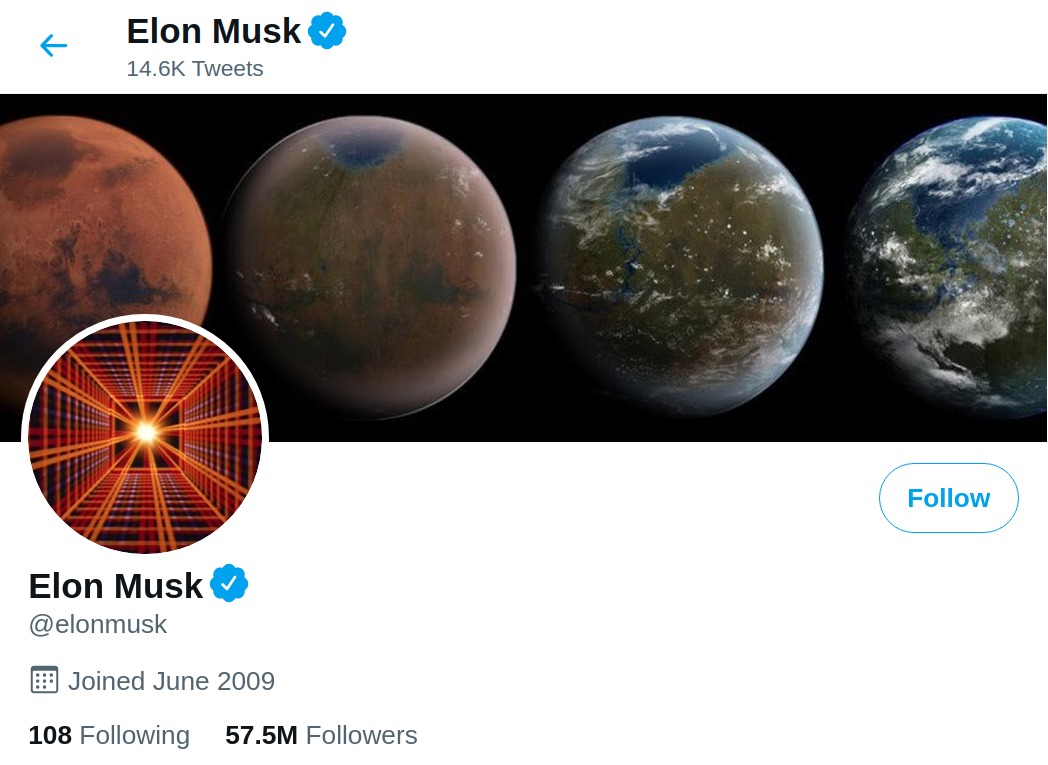
\includegraphics[width=0.8\textwidth]{musk_profile.png}
\caption{Screenshot of Elon Musk's Twitter profile on \date{26 June 2021}, see \url{https://twitter.com/elonmusk?lang=en}.}
\label{fig:twitter_musk}
\end{figure}

\subsection{Twitter Activity}

Fig.~\ref{fig:twitter_musk} contains a screenshot of Elon Musk's Twitter profile from \date{26 June 2021}. At that date, the Twitter profile has $57.5$ million followers, and follows $108$ other Twitter users. The typical format of a Tweet is depicted in Fig.~\ref{fig:example_tweet}. A Tweet consists of a text of up to $280$ characters, and may contain URLs, referals to other Twitter users, photos, or videso. Other Twitter users can share their reaction to the Tweet by liking, Retweeting or replying to it. A Retweet shows the Tweet on the profile of the Retweeting user, and is somewhat comparable to forwarding e-mails. \\

\begin{figure}[h!]
\centering
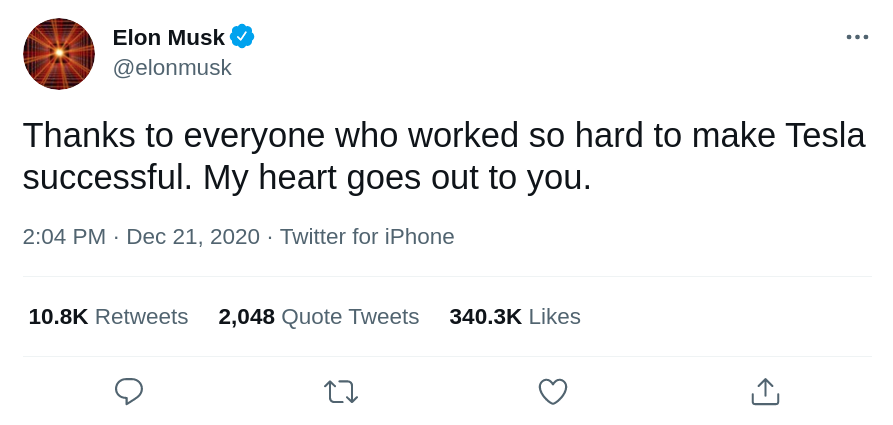
\includegraphics[width=0.8\textwidth]{example_tweet.png}
\caption{Screenshot of an examplary Elon Musk Tweet on \date{21 December 2020}, see \url{https://twitter.com/elonmusk/status/1341006575650140161}. Each Tweet consists of a text of up to $280$ characters, and may contain URLs, referals to other Twitter users, photos, or videos. Other Twitter users can like the Tweet, reply to it, and Retweet it.}
\label{fig:example_tweet}
\end{figure}

\SI{10.00}{\percent} of Elon Musk's Tweets contain URLs to other websites (that may be simply another part of Twitter). \SI{5.66}{\percent} of his Tweets contain photos, and \SI{6.81}{\percent} embed videos. A Tweet is not necessarily an independent text, but may refer to another Tweet. This type of Tweet is called reply. \SI{64.27}{\percent} of Elon Musk's Tweets are replies to other Twitter users, showing a strong interaction with the Twitter community. \\

\begin{figure}[h!]
\centering
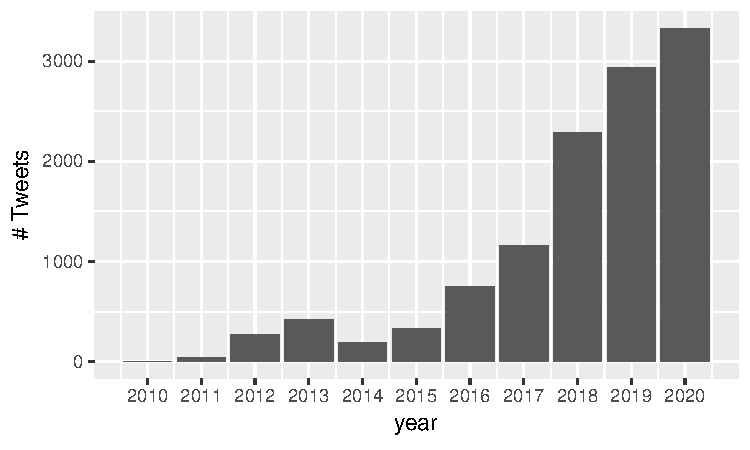
\includegraphics[width=0.8\textwidth]{tweets_per_year.pdf}
\caption{Total number of Tweets published by Elon Musk per year from 2010 to 2020. The barplot reveals a continuous increase of posted Tweets per year. In total, Elon Musk published $11717$ Tweets in the reported time period.}
\label{fig:tweets_per_year}
\end{figure}

Fig.~\ref{fig:tweets_per_year} reports the total number of Tweets posted by Elon Musk per year. A continuous increase from the year 2010 to 2020 is observable. In the same time period the reactions of other Twitter users on his Tweets has increased, as is shown in Fig.~\ref{fig:likes_replies_retweets}. The Figure displays the average number of likes, replies, and Retweets on Elon Musk's Tweets for each year. The reported uncertainties are the standard error on the average. As there is only one Tweet in 2010, no uncertainty is displayed for that year.

\begin{figure}[h!]
\centering
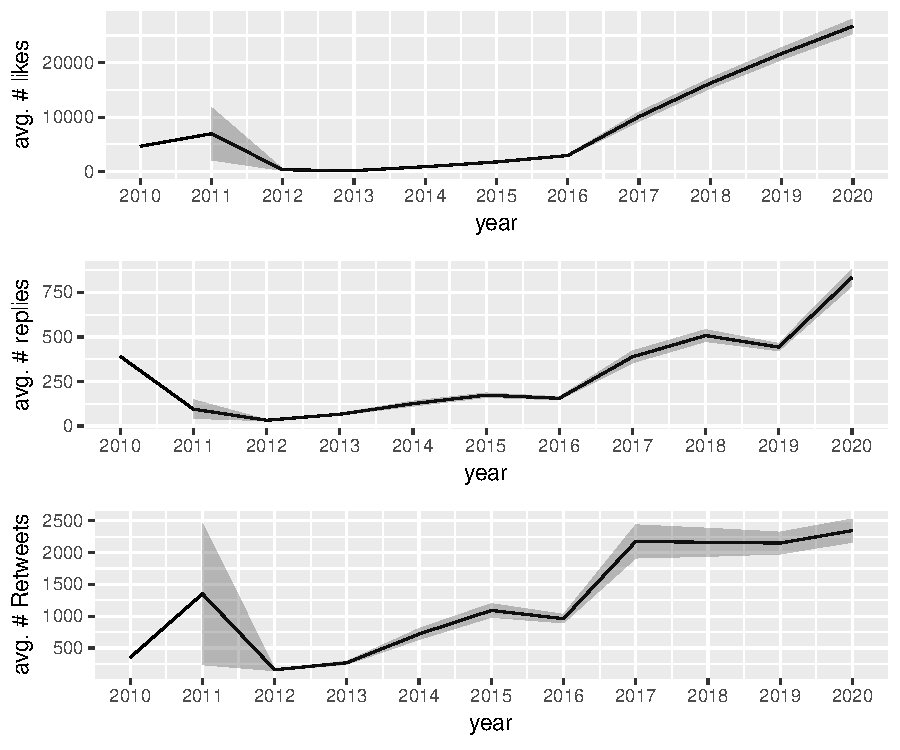
\includegraphics[width=0.8\textwidth]{likes_replies_retweets.pdf}
\caption{Average number of likes, replies, and Retweets on Elon Musk's Tweets per year. The displayed uncertainties are the standard error of the average. For 2010, no standard error is computed as Elon Musk published only one Tweet in this year. Parallel to Elon Musk's increasing Twitter activity over the years observed in Fig.~\ref{fig:tweets_per_year}, also the average number of likes, replies, and Retweets grows.}
\label{fig:likes_replies_retweets}
\end{figure}

Elon Musk's activity on Twitter is roughly equally distributed over the $24$ hours of a day apart from a drop in the morning hours between $2$ AM and $7$ AM, see Fig.~\ref{fig:tweets_per_hour}. The time refers to the pacific day time (PDT) which is the time zone of Elon Musk's home state California. 

\begin{figure}[h!]
\centering
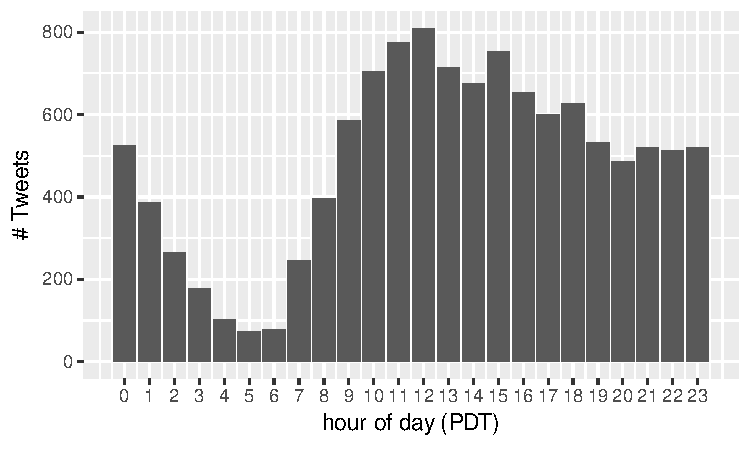
\includegraphics[width=0.8\textwidth]{tweets_per_hour.pdf}
\caption{Total number of Tweets published by Elon Musk per hour of the day, which refers to pacific day time (PDT) - the time zone of Elon Musk's home state California. The Tweets are almost equally distributed over all hours of the day apart from a drop during the morning hours from $2$ AM to $7$ AM.}
\label{fig:tweets_per_hour}
\end{figure}

\subsection{Interaction with Other Users \& Websites}

As already explained above, \SI{64.27}{\percent} of Elon Musk's Tweets are replies to other Twitter users. First insights on Elon Musk's interests may be gained by analyzing the Twitter users that he mentions  most often. An ordered barplot of these users can be found in Fig.~\ref{fig:users}. His main interest seems to be @Tesla and related accounts like @Teslarati, and @teslaownersSV. Secondly, @SpaceX and space-related users such as @Erdayastronaut, @NASASpaceflight, and the US space agency @NASA appear commonly.\\

Another source of information are the URLs in Elon Musk's Tweets. In total, \SI{10.00}{\percent} of his Tweets until the end of 2020 contain URLs. The corresponding barplot is reported in Fig.~\ref{fig:urls}. Note that only the domain name is reported as the focus lies on the detection of general interests. For this purpose, the analysis of specific URLs is not suitable, and would not be visualizable as a barplot. First of all, he commonly refers to social networks like Twitter itself, Youtube, and Instagram. This illustrates that he is also active (at least passively) on these platforms. Again, several URLs refer to Tesla. URLs containinig SpaceX are less common. Additionally, Elon Musk appears to be informed on economic topics as his referals to Bloomberg, Buiseness Insider, and the Wall Street Journal show.

\begin{figure}[h!]
\centering
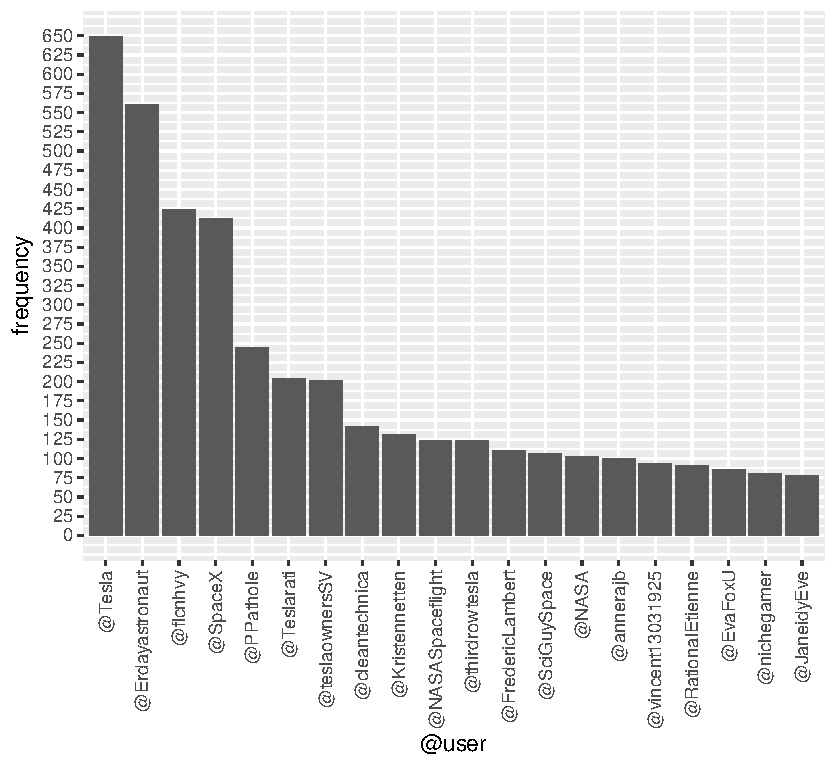
\includegraphics[width=0.8\textwidth]{users.pdf}
\caption{Frequency of referals to other Twitter users that are mentioned in at least $75$ Tweets. In total, \SI{64.27}{\percent} of Elon Musk's Tweets until the end of 2020 are replies to other Twitter users. Note, however, that referals to other Twitter users (@user) are also possible in Tweets that are not a direct reply. The interaction with Twitter accounts related to @Tesla is striking. In addtion, an interest in @SpaceX as well as space related users like @Erdayastronaut, @NASASpaceflight, and the US space agency @NASA is observed.}
\label{fig:users}
\end{figure}

\clearpage

\begin{figure}[h!]
\centering
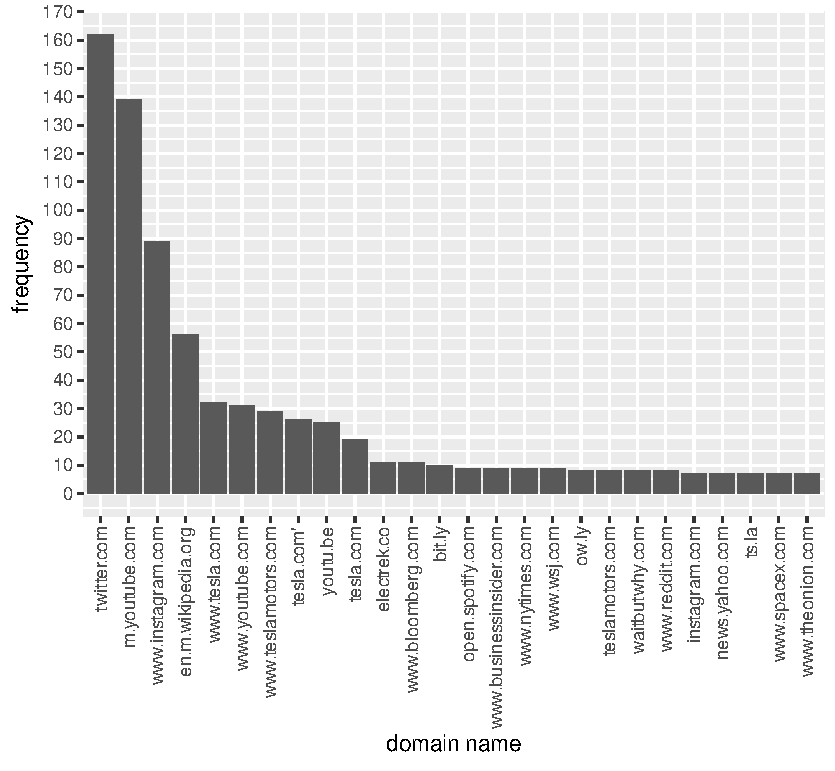
\includegraphics[width=0.8\textwidth]{urls.pdf}
\caption{Frequency of referals to other websites that are mentioned in at least $6$ Tweets. In total, \SI{10.00}{\percent} of Elon Musk's Tweets until the end of 2020 contain URLs. Apart from the domains of social networks like Twitter itself, YouTube, and Instagram, again the interest in Tesla is striking. Elon Musk also seems to be up to date on economic related topics as his referals to Bloomberg, Buiseness Insider, and Wall Street Journal show.}
\label{fig:urls}
\end{figure}

\subsection{Tweet Preprocessing \& Word Usage}

For the application of unsupervised clustering techniques in the following part of the present work, the text of the Tweets in the Kaggle dataset is preprocessed. The preprocessing consists in the following steps:

\begin{itemize}
\item The removal of all URLs and Twitter user names as they were already inspected above, and the following analysis is based on actual words in the Tweets.
\item The transformation of all words to lower case because the analysis should not make a difference between upper and lower case words like \enquote{Tesla} and \enquote{tesla}.
\item The removal of common stopwords, as reported in Fig.~\ref{fig:stopwords_en} and Fig~\ref{fig:stopwords_smart} in the Appendix. Stopwords are words that appear commonly in (english) texts, and are thus not helpful in clustering the Tweets as they do not add meaning but have mostly a grammatical function.
\item The removal of punctuation like dots, commas, and exclamation points.	
\item The removal of numerical digits like \enquote{12} and \enquote{7}.
\end{itemize}

After the preprocessing, the remaining text of each Tweet is a sequence of words (that are not stopwords). All of the Tweets together contain $11572$ different words (that may occur multiple times). In Fig.~\ref{fig:word_count}, the frequency of the most common words in all preprocessed Tweets is reported. Again, the word \enquote{tesla} occurs frequently. Other common words are \enquote{car(s)} and \enquote{model}. Besides general terms, referals to rockets and space like \enquote{rocket}, \enquote{spacex}, \enquote{Mars}, and \enquote{launch} appear in several Tweets.

\begin{figure}[h!]
\centering
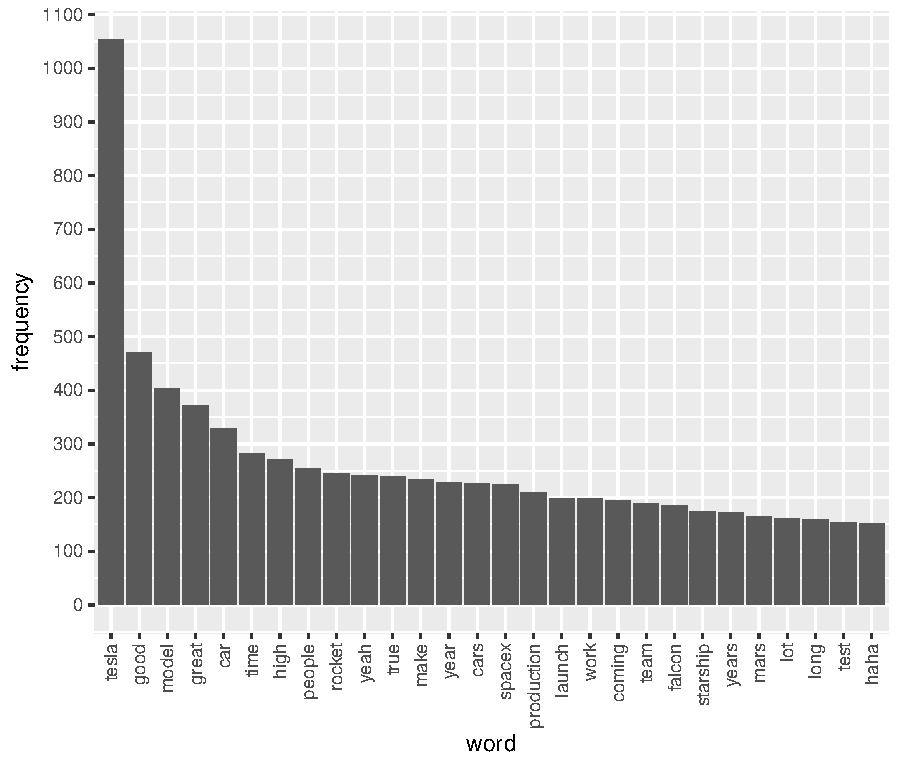
\includegraphics[width=0.8\textwidth]{word_count.pdf}
\caption{Frequency of words in Elon Musk's Tweets that occur at least $150$ times. In total, all Tweets contain $11572$ different words after the application of the stopword lists in Fig.~\ref{fig:stopwords_en} and Fig~\ref{fig:stopwords_smart} in the Appendix. Striking is again the heavy usage of the word \enquote{tesla}. In addition, the words \enquote{car(s)}, and \enquote{model} occur frequently. Besides more general terms such as \enquote{good}, and \enquote{true}, several words refering to rockets and space occur, e.g. \enquote{rocket}, \enquote{spacex}, \enquote{Mars}, and \enquote{launch}.}
\label{fig:word_count}
\end{figure}